\chapter{Resultados}\label{chp:resultados}
\vspace{-1.5cm}
\noindent\rule{\columnwidth}{1.2mm}
\vspace{0.1cm}

\section{Resultados Obtidos}

Ao aplicar o método da área do edifício, obteve-se os valores da densidade de potência de iluminação limite para cada nível energético, da edificação estudada, com base nas especificações do RTQ-C, para a atividade principal Escola/Universidade, da Tabela \ref{tab1}. Vale ressaltar que a edificação possui uma área total de 5892,12 $m^2$, multiplicando-a pelos coeficientes da Tabela \ref{tab1}, encontrou-se os valores mostrados na Tabela \ref{tab_dpil}.

\begin{table}[H]
\centering
\caption{Valores das potências limites para cada nível, da edificação estudada.}
\label{tab_dpil}
\begin{tabular}{ll}\hline
Nível Energético & Potência (W) \\\hline
A                & 63045,684        \\
B                & 72473,076        \\
C                & 81900,468        \\
D                & 91327,86   \\\hline     
\end{tabular}
\end{table}

Com o trabalho realizado em campo, detectou-se certas características do sistema de iluminação da edificação analisada. Primeiramente, constatou-se que a edificação não atende ao critério de desligamento automático do sistema de iluminação, e isso já inviabiliza a obtenção da ENCE parcial de nível A para essa edificação. A edificação, em alguns ambientes, não atende ao critério da contribuição da luz natural em sua totalidade, uma vez que observou-se que em algumas salas, as janelas possuem películas de controle solar, que dificulta a entrada a luz natural no ambiente, e também, em certos ambientes, a fileira de luminárias próximas à janela, não possuem um controle para acionamento independente, que faz com que as lâmpadas fiquem acesas mesmo com a entrada da luz natural no ambiente, e esse fator, combinado com o não atendimento do critério de desligamento automático do sistema de iluminação, inviabiliza que a edificação receba uma ENCE parcial de nível A e de nível B para o sistema de iluminação.

Porém, a edificação apresentou alguns aspectos positivos, constatou-se que em todos os ambientes, o critério da divisão de circuitos é atendido. Observou-se também que algumas medidas para a redução do consumo energético foram tomadas, em uma ala do segundo pavimento da edificação, as lâmpadas utilizadas são de LED com potência de 18 W, com luminárias que utilizam 2 lâmpadas apenas, e em grande parte do edifício, as lâmpadas instaladas, são fluorescentes de 32 W, com luminárias que utilizam apenas 2 lâmpadas.

Vale ressaltar que, a edificação passou por uma reforma, e possui alguns ambientes, que ainda utilizam lâmpadas incandescentes de 40 W, com luminárias que utilizam 4 lâmpadas. Os ambientes construídos na reforma, são os que apresentam as medidas de redução de consumo energético descrito anteriormente.

Para medir o valor da potência total instalada, realizou-se uma contagem do número de lâmpadas utilizadas em cada ambiente da edificação, levando em consideração o tipo de lâmpada e a potência de cada lâmpada instalada. As Tabelas \ref{tab_terreo}, \ref{tab_pav1} e \ref{tab_pav2}, mostram os valores das potências instaladas de cada ambiente dos pavimentos do edifício, bem como o valor total da potência instalada em cada pavimento. Os ambientes descritos são mostrados nas plantas do edifício, que são mostradas nas Figuras \ref{pav_terreo}, \ref{pav2} e \ref{pav3}, que representam os pavimentos térreo, segundo pavimento e terceiro pavimento, respectivamente. 



\begin{table}[H]
\centering
\caption{Potência instalada do Pavimento Térreo.}
\label{tab_terreo}
\begin{tabular}{ll}\hline
Ambiente                   & Potência(W) \\\hline
Sala 1021                  & 384         \\
Sala 1022                  & 384         \\
Sala 1023                  & 384         \\
Sala 1024                  & 384         \\
Sala 1025                  & 384         \\
Sala 1026                  & 384         \\
Sala 1027                  & 384         \\
Corredor1                  & 1408        \\
Hall                       & 448         \\
Copa                       & 320         \\
Almoxarifado Tec. Elétrica & 160         \\
Sala 1001                  & 1280        \\
Sala 1002                  & 1280        \\
Sala 1003                  & 1280        \\
Sala 1004                  & 1280        \\
Sala 1005                  & 1280        \\
Corredor2                  & 1600        \\
Sala 1006/1007             & 1920        \\
Sala 1008                  & 960         \\
Sala 1009/1010             & 1920        \\
Banheiro Masc.             & 240         \\
Banheiro Fem.              & 160         \\
Escada                     & 160         \\\hline
Total                      & 18384  \\\hline    
\end{tabular}
\end{table}

\begin{table}[H]
\centering
\caption{Potência instalada do Segundo Pavimento.}
\label{tab_pav1}
\begin{tabular}{ll}\hline
Ambiente       & Potencia (W) \\\hline
Sala 1011      & 1280         \\
Sala 1012      & 1280         \\
Sala 1013      & 1280         \\
Sala 1014      & 1280         \\
Sala 1015/1016 & 2560         \\
Sala 1017      & 1280         \\
Sala 1018      & 1280         \\
Sala 1019      & 1280         \\
Sala 1020      & 1280         \\
Corredor 3     & 1440         \\
Hall           & 384          \\
Sala MM1       & 324          \\
Sala MM2       & 324          \\
Sala MM3       & 324          \\
Sala MM4       & 324          \\
Sala MM5       & 324          \\
Secret. TRU    & 144          \\
Secret. CIV    & 144          \\
Secret. GERAL  & 360          \\
Secret. ELE    & 144          \\
Secret. ARQ    & 144          \\
Colegiado      & 108          \\
Lig 1          & 324          \\
Lig 2          & 324          \\
Informática    & 144          \\
L.A.U          & 324          \\
Banheiro Masc. & 240          \\
Banheiro Fem.  & 240          \\
Escada         & 160          \\
Corredor 4     & 540          \\
Almoxarifado   & 80           \\\hline
Total          & 19664  \\\hline       
\end{tabular}
\end{table}


\begin{longtable}[H]{ll}
\caption{Potência instalada do Terceiro Pavimento.}
\label{tab_pav2}\\\hline
Ambiente & Potencia (w) \\\hline
\endfirsthead
%
\endhead
%
Sala MM 6 & 576 \\
Sala MM 7 & 576 \\
Sala MM 8 & 576 \\
Sala MM 9 & 576 \\
Sala MM 10 & 576 \\
Sala MM 11 & 576 \\
Secret. Pós-Grad. & 192 \\
Ambiente & Potencia (w) \\\hline
Acervo Pós-Grad. & 192 \\
Pós-Grad & 384 \\
Pós-Grad & 384 \\
Lab. Doc. & 192 \\
NEPEA & 1024 \\
Corredor 5 & 1152 \\
Hall & 400 \\
Copa & 320 \\
Corredor 6 & 1344 \\
Docente ELE 1 & 256 \\
Docente ELE 2 & 256 \\
Docente ELE 3 & 256 \\
Docente ELE 4 & 256 \\
Docente ELE 5 & 256 \\
Docente ELE 6 & 256 \\
Docente ELE 7 & 256 \\
Docente ELE 8 & 256 \\
Docente ELE 9 & 256 \\
Docente CIV 1 & 256 \\
Docente CIV 2 & 256 \\
Docente CIV 3 & 256 \\
Docente CIV 4 & 256 \\
Docente CIV 5 & 256 \\
Docente CIV 6 & 256 \\
Docente CIV 7 & 256 \\
Docente CIV 8 & 256 \\
Docente CIV 9 & 256 \\
Reuniões 1 & 512 \\
Reuniões 2 & 256 \\
Docente TRU 1 & 256 \\
Docente TRU 2 & 256 \\
Docente TRU 3 & 256 \\
Docente TRU 4 & 256 \\
Docente TRU 5 & 256 \\
Docente TRU 6 & 256 \\
Docente ARQ 1 & 256 \\
Docente ARQ 2 & 256 \\
Ambiente & Potencia (w) \\\hline
Docente ARQ 3 & 256 \\
Docente ARQ 4 & 256 \\
Docente ARQ 5 & 256 \\
Docente ARQ 6 & 256 \\
Docente ARQ 7 & 256 \\
Docente ARQ 8 & 256 \\
Docente ARQ 9 & 256 \\
Docente ARQ 10 & 256 \\
Banheiro Masc. & 240 \\
Banheiro Fem. & 240 \\
Escada & 80 \\\hline
Total: & 19072\\\hline
\end{longtable}

Com base nas Tabelas \ref{tab_terreo}, \ref{tab_pav1} e \ref{tab_pav2}, obteve-se que o valor total da potência instalada é de 59856 W, ao comparar com os valores limites obtidos, mostrados na Tabela \ref{tab_dpil}, nota-se que a edificação está apta a receber uma ENCE parcial de nível A, analisando a potência total da edificação. Porém a edificação, como foi dito anteriormente, não atende à um dos pré-requisitos previstos para o sistema de iluminação no RTQ-C, o de desligamento automático do sistema de iluminação, e atende parcialmente ao critério de luz natural. Com base nessas informações, deve-se fazer uma ponderação entre os níveis de eficiência e potência instalada dos ambientes que não atenderam aos pré-requisitos e a potência instalada e o nível de eficiência encontrado para o sistema de iluminação.

Levando em consideração que nenhum dos pavimentos atende ao critério de desligamento automático do sistema de iluminação, e que o critério de luz natural é atendido em parte do edifício, e também que a edificação atende em sua totalidade, ao critério de divisão de circuitos, a edificação teria uma ENCE parcial de nível C. No entanto, fazendo a ponderação com a potência instalada em cada pavimento, observando as Tabelas \ref{tab_dpil2} e \ref{tab_pavs}, pode-se ver que a potência instalada de nenhum dos pavimentos, ultrapassa a potência limite, para os pavimentos, do nível A, logo, pode-se dizer que a ENCE parcial final da edificação é de nível B.


\begin{table}[H]
\centering
\caption{Valores das potências limites para cada nível, por pavimentos.}
\label{tab_dpil2}
\begin{tabular}{ll}\hline
Nível Energético & Potência Limite (W) \\\hline
A                & 21015,23            \\
B                & 24157,69            \\
C                & 27300,16            \\
D                & 30442,62     \\\hline      
\end{tabular}
\end{table}


\begin{table}[H]
\centering
\caption{Valores das potências intaladas por pavimento.}
\label{tab_pavs}
\begin{tabular}{ll}\hline
Pavimento          & \begin{tabular}[c]{@{}l@{}}Potência instalada\\   (W)\end{tabular} \\\hline
Pavimento Térreo   & 18384                                                              \\
Segundo Pavimento  & 19664
                                                             \\
Terceiro Pavimento & 19520     \\\hline                                                        
\end{tabular}
\end{table}

\section{Projeções de Melhorias}

Analisando o segundo pavimento da edificação, conforme foi constatado, em uma ala do pavimento, a lâmpadas utilizadas são de LED, com potência de 18 W, e a outra ala, de mesma área, possuem lâmpadas incandescentes, com potência de 40 W. Como pode-se observar, nas Tabelas \ref{tab_40w} e \ref{tab_led}, e no gráfico da Figura \ref{graph2}, a ala que utiliza lâmpadas incandescentes, possui uma potência instalada muito maior, cerca de 66\% maior, que a ala que possui lâmpadas de LED, e consequentemente, uma menor eficiência energética. Vale a pena ressaltar que, na ala que possui lâmpadas incandescentes instalada, a potência instalada, representa cerca de 72\% da potência total do pavimento.



\begin{table}[H]
\centering
\caption{Potência instalada da ala que utiliza lâmpadas incandescentes de 40 W.}
\label{tab_40w}
\begin{tabular}{ll}\hline  
Ambiente       & Potência instalada (W) \\\hline  
Sala 1011      & 1280                   \\
Sala 1012      & 1280                   \\
Sala 1013      & 1280                   \\
Sala 1014      & 1280                   \\
Sala 1015/1016 & 2560                   \\
Sala 1017      & 1280                   \\
Sala 1018      & 1280                   \\
Sala 1019      & 1280                   \\
Sala 1020      & 1280                   \\
Corredor 3     & 1440                   \\\hline  
Total          & 14240  \\\hline                 
\end{tabular}
\end{table}

\begin{table}[H]
\centering
\caption{Potência instalada da ala que utiliza lâmpadas de LED de 18 W.}
\label{tab_led}
\begin{tabular}{ll}\hline  
Ambiente      & Potência instalada (W) \\\hline  
Sala MM1      & 324                    \\
Sala MM2      & 324                    \\
Sala MM3      & 324                    \\
Sala MM4      & 324                    \\
Sala MM5      & 324                    \\
Secret. TRU   & 144                    \\
Secret. CIV   & 144                    \\
Secret. GERAL & 360                    \\
Secret. ELE   & 144                    \\
Secret. ARQ   & 144                    \\
Colegiado     & 108                    \\
Lig 1         & 576                    \\
Lig 2         & 576                    \\
Informática   & 144                    \\
L.A.U         & 324                    \\
Corredor 4    & 540                    \\\hline  
Total         & 4824      \\\hline              
\end{tabular}
\end{table}

\begin{figure}[H]
\centering
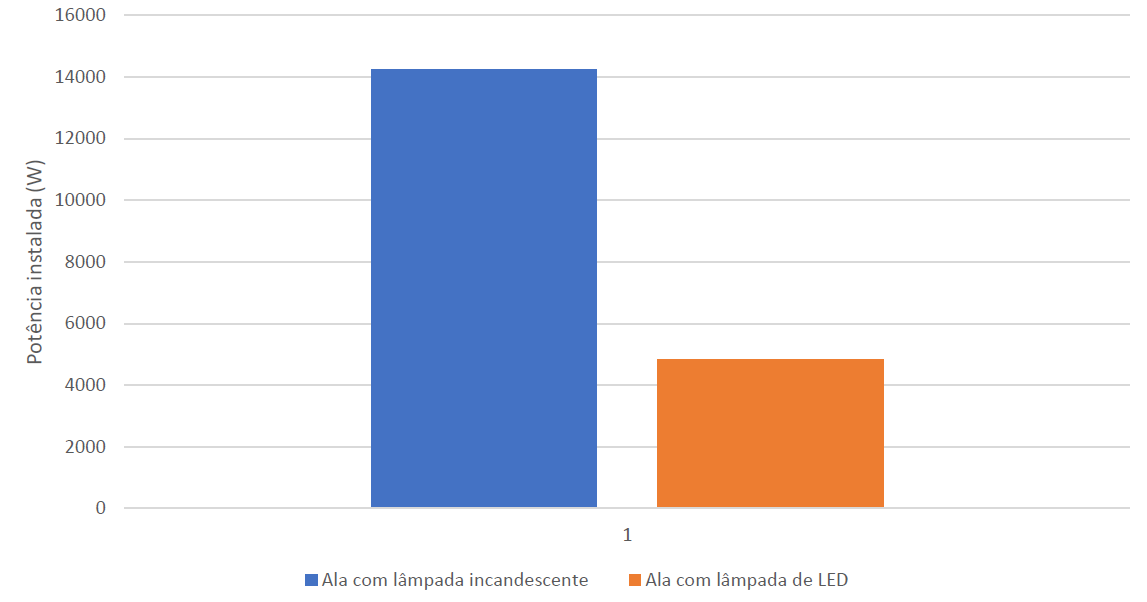
\includegraphics[width = 1.1\textwidth]{Figuras/graph2.PNG}
\caption{Gráfico da comparação entre os valores da potência atual instalada das alas que usam lâmpadas incandescentes e de LED.}
\label{graph2}
\end{figure}


Ao substituir todas as lâmpadas da edificação, por lâmpadas de LED com potência de 18 W, tomando como base as lâmpadas já instaladas na edificação, com luminárias, que utilizam apenas 2 lâmpadas, tem-se uma redução significativa da potência instalada da edificação, conforme mostra a Tabela \ref{tab_proj}.

\begin{table}[H]
\centering
\caption{Tabela de projeções da potência instalada com a alteração sugerida.}
\label{tab_proj}
\begin{tabular}{ll}\hline  
Pavimento          & \begin{tabular}[c]{@{}l@{}}Potência instalada\\   (W)\end{tabular} \\\hline  
Pavimento Térreo   & 7164                                                               \\
Segundo Pavimento  & 8388                                                               \\
Terceiro Pavimento & 10044                                                              \\\hline  
Total              & 25596                \\\hline                                               
\end{tabular}
\end{table}
O gráfico da Figura \ref{graph1} mostra uma comparação entre potência instalada por pavimento, e a potência total, com o valor da potência que cada pavimento teria, e o total também, com a substituição por lâmpadas de LED, com potência de 18 W. Nota-se que a potência da projeção, é muito menor, que a instalada, sendo que a potência total da projeção representa cerca de 45\% do valor da potência atual instalada, ou seja, a potência será reduzida em torno de 55\% do valor atual.

\begin{figure}[H]
\centering
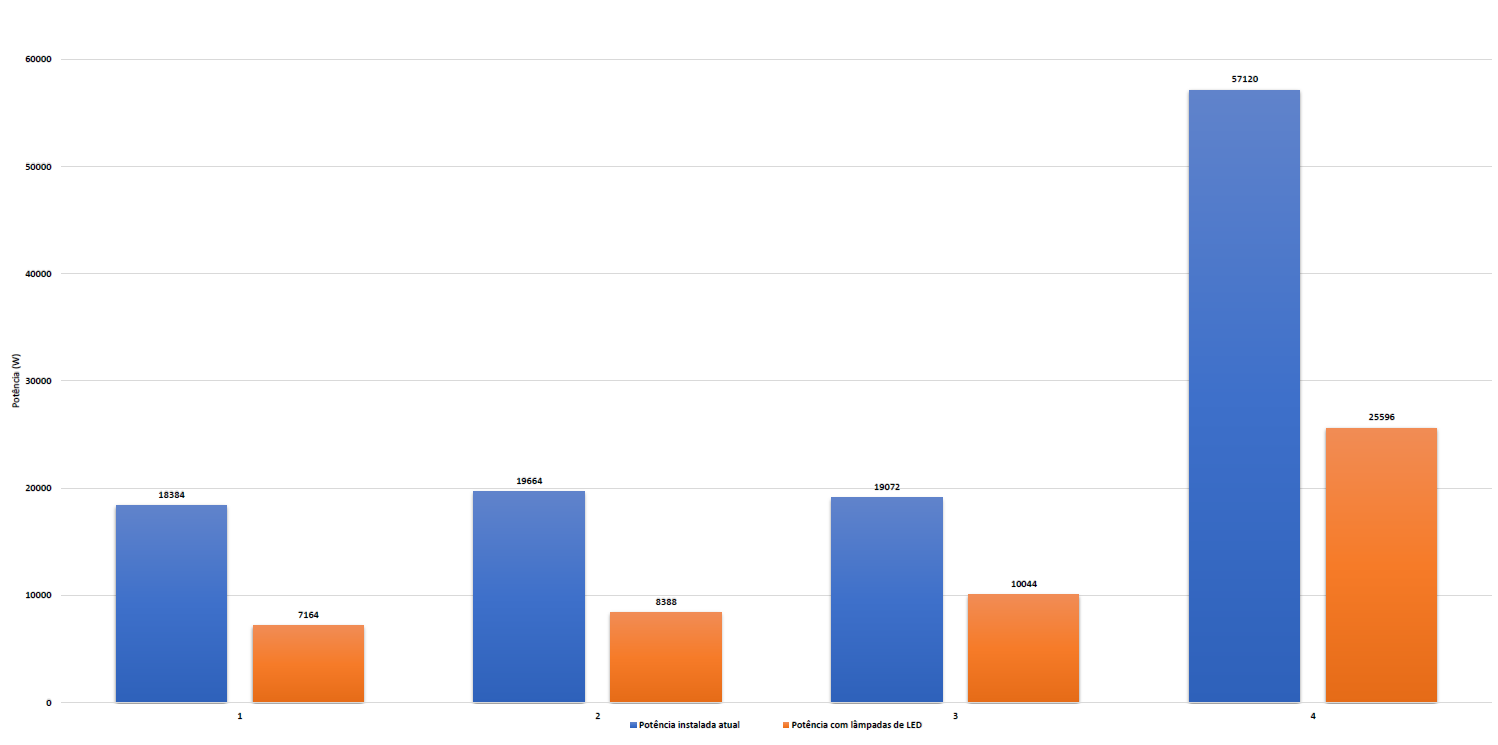
\includegraphics[width = 1.1\textwidth]{Figuras/graph1.PNG}
\caption{Gráfico da comparação entre os valores da potência atual instalada, e a potência de projeção com a alteração sugerida.}
\label{graph1}
\end{figure}


Por pavimento, pode-se observar que, no pavimento térreo, a potência da projeção representa cerca de 39\% da potência atual instalada, sendo reduzida em torno de 61\% ao instalar as lâmpadas de LED. Para o segundo pavimento, a redução é de cerca de 57\%, e para o terceiro pavimento, a redução é de 47\%.

Os valores percentuais de redução da potência instalada variam por pavimento, devido à alguns fatores:
\begin{itemize}
\item No pavimento térreo, grande parte do edifício ainda utiliza lâmpadas incandescentes com potência de 40 W, e luminárias que utilizam 4 lâmpadas, o que resulta em uma grande potência instalada, o que justifica esse alto índice de redução, com a projeção de instalação de lâmpadas de LED;
\item No segundo pavimento, mesmo com uma ala já possuindo a instalação de lâmpadas de LED, a outra ala, como já foi mostrado um comparativo anteriormente, utiliza lâmpadas incandescentes com potência de 40 W, e luminárias que utilizam 4 lâmpadas, o que justifica esse índice de redução;
\item No terceiro pavimento, por ser uma parte da edificação que foi construída após a reforma, conforme foi dito anteriormente, as lâmpadas instaladas são fluorescentes, com uma potência de 32 W, e já possue luminárias que utilizam apenas 2 lâmpadas, e portanto, possue menor índice de redução. 
\end{itemize}

A implementação dessa solução de melhoria, teria um custo, de certa forma, elevado, uma vez que as lâmpadas de LED, possuem um valor elevado, quando comparados aos custos das lâmpadas incandescentes e fluorescentes. Porém, o investimento vale a pena, tendo em vista que, ao longo prazo, esse investimento será compensado no custo do consumo energético da edificação. O sistema de iluminação será muito mais eficiente, o que gerará uma economia no consumo energético, e consequentemente, uma economia no gasto com energia elétrica.

Para atender aos outros pré-requisitos para o sistema de iluminação, previstos no RTQ-C, vê-se necessário, a instalação de um dispositivo de controle, para desligar automaticamente, o sistema de iluminação. A alternativa viável para atender esse critério, seria a implantação de sensores de presença, nos corredores da edificação, uma vez que, no período noturno, a iluminação dos corredores permanece ligada de forma constante, até encerrar toda as atividades do edifício. Esse dispositivo seria programado para desligar o sistema de iluminação após 30 minutos após a saída de todos os ocupantes, conforme prevê o RTQ-C, e ligaria a iluminação ao detectar a presença de alguma pessoa no ambiente. Nos demais ambientes da edificação, não se faz necessário essa implementação, tendo em vista, que as salas de aulas, quando não estão em atividade, o sistema de iluminação não permanece ligado.

Um ponto importante que pode ser melhor utilizado é a questão da luz natural. A luz natural, é um recurso muito importante, que ao ser utilizado de forma correta, gera uma grande economia no consumo de energia elétrica. Uma alteração importante a ser implementada na edificação, é um dispositivo de controle independente, para desligar a fileira de lâmpadas que se localizam próximas à janela. Uma opção interessante, para aproveitar melhor a luz natural nos ambientes, seria a implementação de um sistema de dimerização, que permite ajustar a intensidade luminosa das lâmpadas, podendo assim, ponderar a luz natural que entra no ambiente, com o sistema de iluminação, deixando o ambiente com uma iluminação agradável. Vale a pena ressaltar que, para cumprir ao critério da luz natural, é necessário, além do que foi descrito, realizar o método da simulação.

A implementação das sugestões realizadas, para melhorar a eficiência energética da edificação, apesar de ter um custo elevado, tornaria o edifício mais eficiente, tendo em vista os resultados obtidos do trabalho realizado em campo, ponderando com o resultados das projeções realizadas, a edificação, passaria a atender a todos os pré-requisitos, previstos para o sistema de iluminação no RTQ-C, e como a potência instalada no edifício já é abaixo da potência limite para o nível A, e como mostra as projeções, ainda teria uma redução de 55\% do valor total instalado atualmente, credenciaria a edificação a obter um ENCE parcial para o sistema de iluminação de nível A.



















